

\chapter{Graphics}

\begin{figure}[H]
\centering
\includegraphics[scale=0.4]{img/GR-FR.png}
\caption{Functional requirements for Buildability.}
\label{figure:test}
\end{figure}


\section{Plots}
Plots are preferably done using the package \texttt{pgfplots}. Below is an example given. The example also show how to put figures side-by-side in your document using the \texttt{\textbackslash subfloat} command. Open \texttt{data.txt} in a text editor and have a look at its structure. The \LaTeX{} document reads the data from the text file and produces a plot. Axes are automatically scaled depending on the data range given in the text file. 

%------------------------------------------------------------------------------------
\begin{figure}[H]
\centering
\subfloat[Diagonal components of $\bar{D}$.]{
\begin{tikzpicture}
\begin{axis}[
	scale=0.85, % size of the plot
	every axis/.append style={line width=1pt},
    xlabel = $\bar{\varepsilon}_\text{zz}$,
    ylabel style={align=center},
    ylabel = $D_\text{cp}$,
    y unit = {\si{\kilogram\per\meter\square\second}},
    x unit = -,
    cycle list name=linestyles,
    legend style={cells={anchor=west}},
    legend pos=north west,
    ]
\addplot table[mark=none,x expr=\thisrow{strain},y expr=\thisrow{Dxx}] {datafiles/data.txt};
\addplot table[mark=none,x expr=\thisrow{strain},y expr=\thisrow{Dyy}] {datafiles/data.txt};
\addplot table[mark=none,x expr=\thisrow{strain},y expr=\thisrow{Dzz}] {datafiles/data.txt};
\legend{$(\bar{D})_{xx}$,$(D)_{yy}$,$(D)_{zz}$};
\end{axis}
\end{tikzpicture}
\label{fig:a}
}\hfill % \hfill fills out the space inbetween the plots
\subfloat[Off-diagonal components of $\bar{D}$.]{
\begin{tikzpicture}
\begin{axis}[
	scale=0.85,
	every axis/.append style={line width=1pt},
    xlabel = $\bar{\varepsilon}_\text{zz}$,
    ylabel style={align=center},
    ylabel = $(\bar{D})_\bullet/D_\text{cp}$,
    ylabel style={yshift=-0.2cm},
    y unit = -,
    x unit = -,
    cycle list name=linestyles,
    legend style={cells={anchor=west}},
    legend pos=north west,
    ]
\addplot table[mark=none,x expr=\thisrow{strain},y expr=\thisrow{Dxy}] {datafiles/data.txt};
\addplot table[mark=none,x expr=\thisrow{strain},y expr=\thisrow{Dxz}] {datafiles/data.txt};
\addplot table[mark=none,x expr=\thisrow{strain},y expr=\thisrow{Dyz}] {datafiles/data.txt};
\legend{$(D)_{xy}$,$(\bar{D})_{xz}$,$(\bar{D})_{yz}$};
\end{axis}
\end{tikzpicture}
\label{thelabelcanbeanyingreally}
}
\caption[This is the caption text that goes into the table of contents.]{Components of the macroscale diffusivity tensor, $\bar{D}$, as a function of macroscale strain. Numerical values are normalized with respect to $D_\text{cp}$.}
\label{omg}
\end{figure}
%------------------------------------------------------------------------------------
You can cross-reference to each of the figures in this way: \cref{fig:a} and \cref{thelabelcanbeanyingreally}. You can also plot analytical functions \texttt{pgfplots} as shown in \cref{analytical} below.
%------------------------------------------------------------------------------------
\begin{figure}[H]
\centering
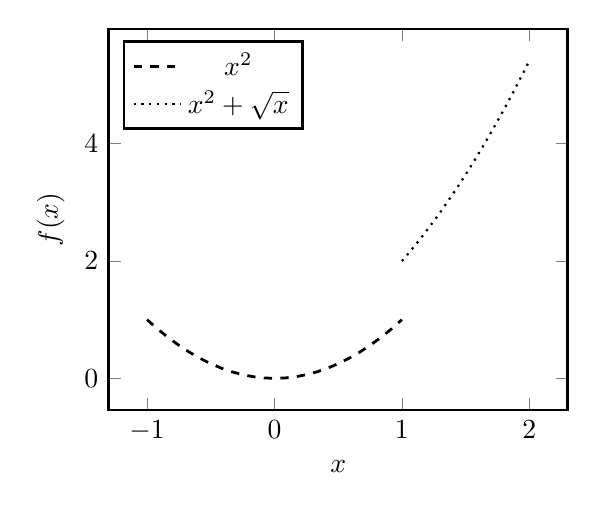
\begin{tikzpicture}
\begin{axis}[	scale=0.85,
every axis/.append style={line width=1pt},
xlabel = $x$,
ylabel = $f(x)$,
legend pos=north west,
]
\addplot[dashed,domain=-1:1]{x^2};
\addplot[dotted,thick,domain=1:2]{x^2 + sqrt(x)};
\legend{$x^2$,$x^2 + \sqrt{x}$}
\end{axis}
\end{tikzpicture}
\caption{Examples of analytical functions.}
\label{analytical}
\end{figure}
%------------------------------------------------------------------------------------

\section{Tables}
Table contents is placed above the table. Vertical lines in tables should be avoided at all cost. Compare the two tables below:
\begin{table}[H]
	\begin{center}
		\caption{An ugly table.} \label{tab:ugly}
		\begin{tabular}{||l|lr||}
			Animal     & Description & Price (\$)\\\hline
			gnats     & gram      & \$13.65 \\ \cline{2-3}
			& each      & .01 \\ \hline
			gnu       & stuffed   & 92.50 \\ \cline{1-1} \cline{3-3}
			emu       &           & 33.33 \\ \hline
			armadillo & frozen    & 8.99 \\ \hline
		\end{tabular}
	\end{center}
\end{table}

\begin{table}[H]
	\begin{center}
		\caption{A beautiful table.} \label{tab:beautiful}
		\begin{tabular}{@{}llr@{}} \toprule
			\multicolumn{2}{c}{Item} \\ \cmidrule(r){1-2}
			Animal & Description & Price (\$)\\ \midrule
			Gnat  & per gram  & 13.65 \\
			& each      & 0.01 \\
			Gnu   & stuffed   & 92.50 \\
			Emu   & stuffed   & 33.33 \\
			Armadillo & frozen & 8.99 \\ \bottomrule
		\end{tabular}
	\end{center}
\end{table}
\Cref{tab:ugly,tab:beautiful} provide the same information. However, \cref{tab:beautiful} is much easier to read simply because it is typeset differently. As you can tell, the vertical lines in \cref{tab:ugly} do not help the reader in separating the different columns. Notice how the top and bottom horizontal lines in \cref{tab:beautiful} are thicker than the two other lines in order to mark the beginning and end of the table. The following guidelines apply to tables:
\begin{itemize}
	\setlength\itemsep{0em}
	\item Avoid vertical lines.
	\item Minimize the need for horizontal lines.
	\item Avoid creating boxes around the items in the table.
	\item Units should be places in the column heading.
	\item The caption of a table should be printed above the table, as opposed to under (as for figures).
\end{itemize}
